%\documentclass[iop]{emulateapj}
% \documentclass[12pt, preprint]{emulateapj}
%\documentclass[twocolumn,amsmath,aps,prd,preprintnumbers,amssymb,nofootinbib,superscriptaddress,showpacs,floatfix]{revtex4-1}
\documentclass[12pt, onecolumn]{emulateapj}

\usepackage{amsmath}
\usepackage{multirow}
\usepackage{array}
%\usepackage{bibtex}
%\bibliographystyle{unsrtnat}

%yellow, orange, red, red!50!blue, blue, green
\usepackage{tikz}
\usetikzlibrary{fit}

\tikzstyle{data} = [rectangle, text centered, draw=black, fill=black!20]
\tikzstyle{prior} = [rectangle, text centered, draw=black, fill=blue!20]
\tikzstyle{selection} = [rectangle, text centered, draw=black, fill=blue!20]
\tikzstyle{posterior} = [rectangle, text centered, draw=black, fill=black!20]
\tikzstyle{full} = [rectangle, text centered, draw=black, fill=black!20]
\tikzstyle{final} = [rectangle, text centered, draw=black, fill=green!20]
\tikzstyle{model} = [rectangle, rounded corners, text centered, draw=black, fill=red!20]
\tikzstyle{params} = [rectangle, rounded corners, text centered, draw=black, fill=yellow!20]
\tikzstyle{arrow} = [thick,->,>=stealth]

\newcommand{\myemail}{aimalz@nyu.edu}
\newcommand{\textul}{\underline}
\newcommand{\scippr}{\texttt{scippr}}

\newcommand{\RN}[1]{%
	\textup{\uppercase\expandafter{\romannumeral#1}}%
}

\newcommand\MyBox[2]{
  \fbox{\lower0.75cm
    \vbox to 3.5cm{\vfil
      \hbox to 3.5cm{\hfil\parbox{3.2cm}{#1\\#2}\hfil}
      \vfil}%
  }%
}

%\slugcomment{}

\shorttitle{Probabilistic inference of the Hubble parameter}
\shortauthors{Malz, Peters, Hlo\v{z}ek, et al.}

\begin{document}
\newcommand{\tkTP}[1]{\textcolor{red}{#1}}  % Tina
\newcommand{\tkRH}[1]{\textcolor{blue}{#1}}  % Renee
\newcommand{\tkAM}[1]{\textcolor{green}{#1}}  % Alex  
\title{Supernova Cosmology Inference with Probabilistic Photometric Redshifts}

\author{Alex Malz\altaffilmark{1}}
\author{Tina Peters\altaffilmark{2}}
\author{Ren\'ee Hlo\v{z}ek\altaffilmark{2}}
\author{Humna Awan}
\author{Anita Bahmanyar\altaffilmark{2}}
\author{Lluis Galbany}
\author{Boris Leistedt\altaffilmark{1}}
\author{Kara Ponder}
\altaffiltext{1}{Center for Cosmology and Particle Physics, Department of Physics, New York University, 726 Broadway, 9th floor, New York, NY 10003, USA}
\altaffiltext{2}{Dunlap Institute \& Department of Astronomy and Astrophysics, University of Toronto, 50 St George Street, Toronto, ON M5S 3H4 Canada}
\email{aimalz@nyu.edu}

\begin{abstract}
The BEAMS framework employs probabilistic supernova classifications to estimate the Hubble parameter that quantifies the relationship between distance and redshift over cosmic time.  This work extends BEAMS to replace high-confidence spectroscopic redshifts with probabilistic photometric redshifts, enabling inference of the Hubble parameter as a function of two probabilistic variables.  By combining posterior probabilities of supernova type and posterior probabilities of host galaxy redshift, we infer a posterior probability distribution over the redshift-dependent Hubble parameter.  This work also produces the \scippr code that can be used to infer cosmological parameters from probabilistic supernova fit parameters.
\end{abstract}
\keywords{}
\maketitle

\section{Introduction}
\label{sec:intro}
The future of supernova cosmology is photometric. Ambitious survey telescopes like the Large Synoptic Survey Telescope (LSST) will yield more than two orders of magnitude mode `candidate' supernova detections, a combination of the more cosmologically useful Type Ia supernovae and interlopers of many different sorts of core-collapse events and interesting objects. Over the past decade, work has been intensifying to answer the question: \textit{'How does one perform cosmological analysis on a hetereogenous population of supernovae without certainty in the specific type of any object?'} \citet{kunz_bayesian_2007, kelly_flexible_2008, hlozek_photometric_2012, lochner_2012, newling_2012}

The key concept in the above is a lack of certainty in the specific type. While the sophistication of classification methods as applied to photometric data is improving greatly \cite{classification_papers}, most yield either a classification type `score' or some other proxy for probability of type (eg. from fitting the data to a suite of light curve templates from a specific type).

When selecting a final data set over which to test cosmological models, one then either makes a cut on probability of the Type Ia, or includes all the data in a Bayesian framework \citet{kunz_bayesian_2007, kelly_flexible_2008, hlozek_photometric_2012, lochner_2012, newling_2012}.

Typing probability isn't, however, the only source of systematic that must be considered for photometric surveys. Indeed, photometric redshift uncertainties (and potential biases) are also important when fitting any models to a suite of data. 
Then the question above becomes instead \textit{'How does one perform cosmological analysis on a hetereogenous population of supernovae without certainty in the specific type of any object, or the redshift of the object and its potential host?'}

The problem of inferring the cosmological parameters and redshift-dependent supernova type proportions from purely photometric data in the form of supernova lightcurves and host galaxy photometry is the next hurdle in any rigorous cosmological analysis, one that is beginning to be investigated by the community \cite{lochner_2017}.

Our approach is to infer cosmological parameters and indeed redshift-dependent supernova type proportions purely from photometric candidate (supernova) light curves and host galaxy photometry. We describe the notation in Section~\ref{sec:method} and our method for simulating data in Section~\ref{sec:data}.

\section{Method}
\label{sec:method}


%This work demonstrates a principled approach to inferring cosmological parameters and redshift-dependent supernova type proportions from purely photometric lightcurves of supernovae and host galaxy photometry.  First, we outline the notation used throughout this paper.

Let us consider observations of $N$ supernovae $n$, each with a photometric lightcurve $\textul{\ell}_{n}$ and host galaxy photometry $\vec{f}_{n}$ comprised of fluxes, magnitudes, or colors.  When we conduct a photometric survey, not all supernovae in the universe will make it into our sample due to selection effects; we cannot include observations we did not make, nor do we include those with low confidence or insufficiently complete data.  \textbf{(Actually, I think we can include the low confidence/incomplete data!  The hierarchical model takes care of their impact on the final result.)}  These choices are quantified by nuisance parameters $\vec{\alpha}$ and $\vec{\beta}$ restricting the supernova lightcurves and host galaxy photometry respectively.  

 Every supernova has several intrinsic parameters that are not directly observable: a type $t_{n}$, a redshift $z_{n}$, and a distance modulus $\mu_{n}$.   Traditional methods estimate the values of these parameters from observed lightcurves and host galaxy photometry by assuming that the lightcurves and host galaxy photometry are random variables drawn from distributions that are functions of these unobservable parameters.
 
The unobservable parameters, however, are themselves random variables. The supernova type is a discrete variable, while the redshift $z$ and distance modulus $\mu$ are continuous varibles, drawn from distributions that are themselves functions of some hyperparameters.  

This assumption of the form of the data is implicit when using the types, redshifts, and distance moduli to constrain the cosmological parameters.

As in traditional approaches, we seek to constrain the cosmological parameters comprising $\vec{\Omega}$, among them the Hubble parameter $H_{0}$ and matter density $\Omega_{0}$, and the redshift-dependent type proportions parametrized by $\textul{\phi}$ under some parametrization that need not be specified at this time.  The redshift-dependent type proportions can be thought of as probabilities over type and redshift $p(t, z | \textul{\phi})$.

\subsection{Model}
\label{sec:model}

A hierarchical Bayesian model allows one to estimate the hyperparameters without first inferring the in principle unobservable parameters, as shown in the directed acyclic graph of Fig. \ref{fig:pgm}. This illustrates the relationships between the variables discussed above. It is worth noting that we assume that the parameters associated with supernova $n$ and its host galaxy are statistically independent of the parameters associated with supernova $n'$ and its host galaxy.

\begin{figure*}
\begin{center}
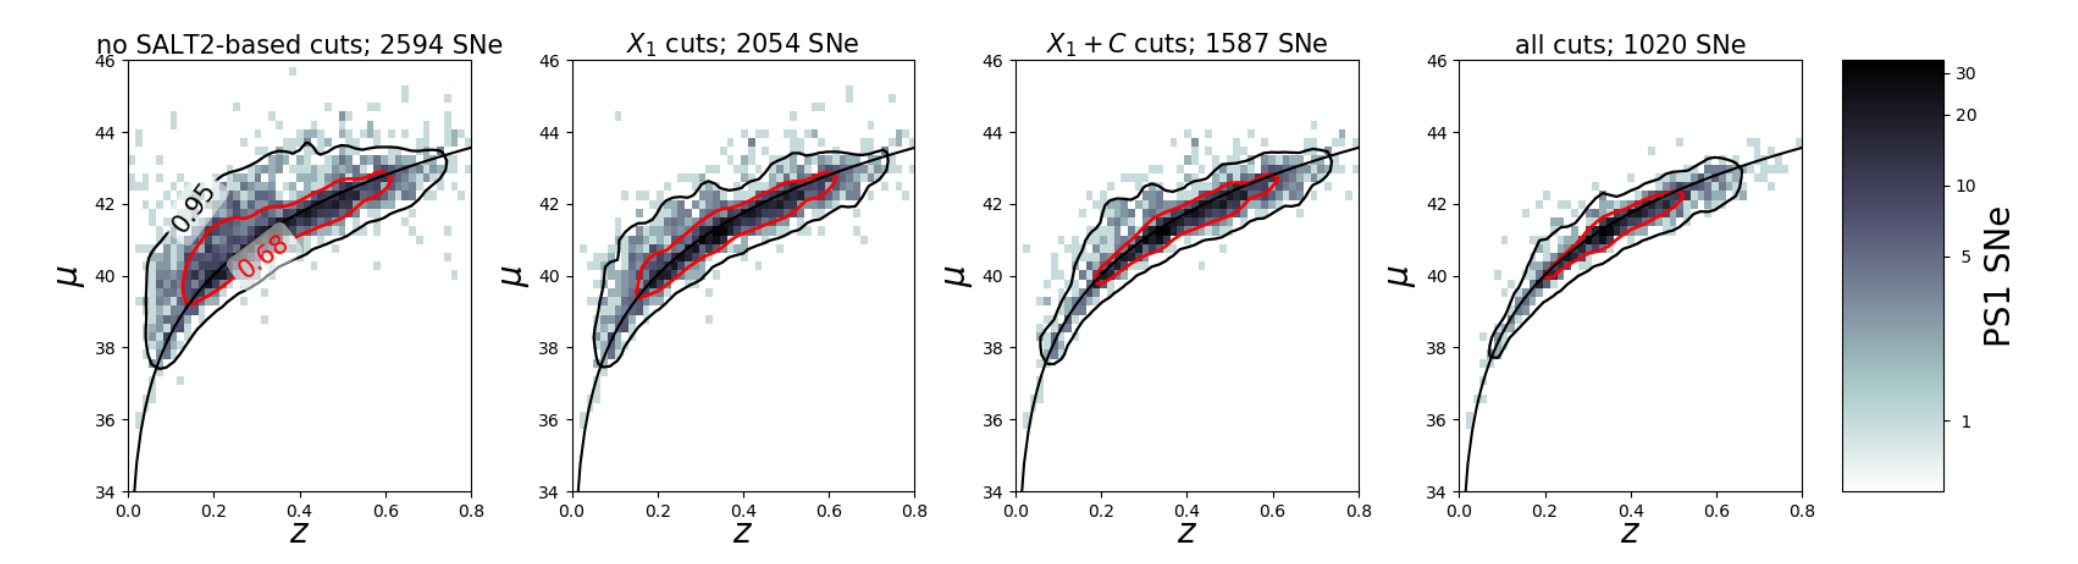
\includegraphics[width=1.0\textwidth]{fig/PanSTARRS.png}
\caption{{\bf Photometric and heterogeneous data:} data from the PanSTARRS survey show the spread in the distance modulus caused by objects with varying type probability. Using cuts reduces this spread, but indeed removes some of the statistical power of the sample. Given faith in a classification algorithm and the resultant purity of the sample, these cuts can be justified, but including all the data weighted by the type probability provides a more robust treatment. Figure from \cite{jones}. \tkRH{[We need some attention grabbing plot rather than the graph to get people's attention!]}
\label{fig:intro}}
\end{center}
\end{figure*}

The motivation for this approach is the existence of photo-$z$ PDFs and the anticipation of PDFs over lightcurve fit parameters, like the colour or stretch in the cast of SALT-II.  Photo-$z$ PDFs are posterior probability distributions; we observe the host galaxy photometry $\vec{f}_{n}$ and learn something about the host galaxy redshift $z_{n}$.  The process by which we derive a relationship between the observed and unobserved parameters imprints its biases in the form of an interim prior that defines a global probability distribution over redshifts parametrized by $\vec{\theta}$.  The selection function also biases the posterior probability in the form of an interim prior parametrized by $\vec{\beta}$.  Thus photo-$z$ PDF is an interim posterior probability distribution $p(z_{n} | \vec{f}_{n}, \vec{\theta}, \vec{\beta})$.

We anticipate the production of lightcurve parameter PDFs, which will also be interim posterior probability distributions, but in a higher dimensional space.  As in the case of photo-$z$ PDFs, the observed multi-band lightcurves $\{\vec{\ell}_{n}\}_{N}$ inform us about the latent parameters of supernova types $\{t_{n}\}_{N}$, redshifts $\{z_{n}\}_{N}$, and distance moduli $\{\mu_{n}\}_{N}$.  The interim prior will be a probability distribution over $t$, $z$, and $\mu$ with known parameters comprising $\textul{\xi}$.  We will also have a lightcurve selection function of parameters $\vec{\alpha}$ that is another distribution over this three-dimensional space.  The overall interim posterior of the supernova lightcurve is then $p(t_{n}, z_{n}, \mu_{n} | \textul{\ell}_{n}, \textul{\xi}, \vec{\alpha})$.
\begin{figure}
\begin{center}
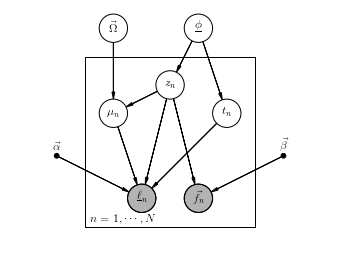
\includegraphics[width=0.55\textwidth]{fig/pgm.png}
\caption{This directed acyclic graph corresponds to a probabilistic graphical model for our hierarchical inference of the cosmological parameters and redshift-dependent type proportion parameters.  In this graph, all random variables are shown in circles, with observed variables shown in shaded circles.  The box indicates that there are $N$ copies of the relationships between boxed parameters, each statistically independent of all others.  The hyperparameters we would like to infer are the cosmological parameters in $\vec{\Omega}$ and the redshift-dependent type proportion parameters comprising $\textul{\phi}$.  Drawn from functions of these hyperparameters are the distance moduli $\{\mu_{n}\}_{N}$, redshifts $\{z_{n}\}_{N}$, and supernova types $\{t_{n}\}_{N}$.  Here, we observe host galaxy colors $\{\vec{f}_{n}\}_{N}$ and multi-band supernova lightcurves $\{\textul{\ell}_{n}\}_{N}$, shown in shaded circles.  The solid dots indicate known constants that factor into the model; $\vec{\alpha}$ represents the parameters defining a selection function in the space of observed lightcurves, and $\vec{\beta}$ includes the parameters defining a selection function in the space of host galaxy photometry.  The arrows encode the relationships between variables, going from parameters defining probability distributions to variables drawn from those probability distributions.}
\label{fig:pgm}
\end{center}
\end{figure}

We illustrate the flow of data through the \scippr process in Figure~\ref{fig:flow1}.
\begin{figure*}
\begin{center}
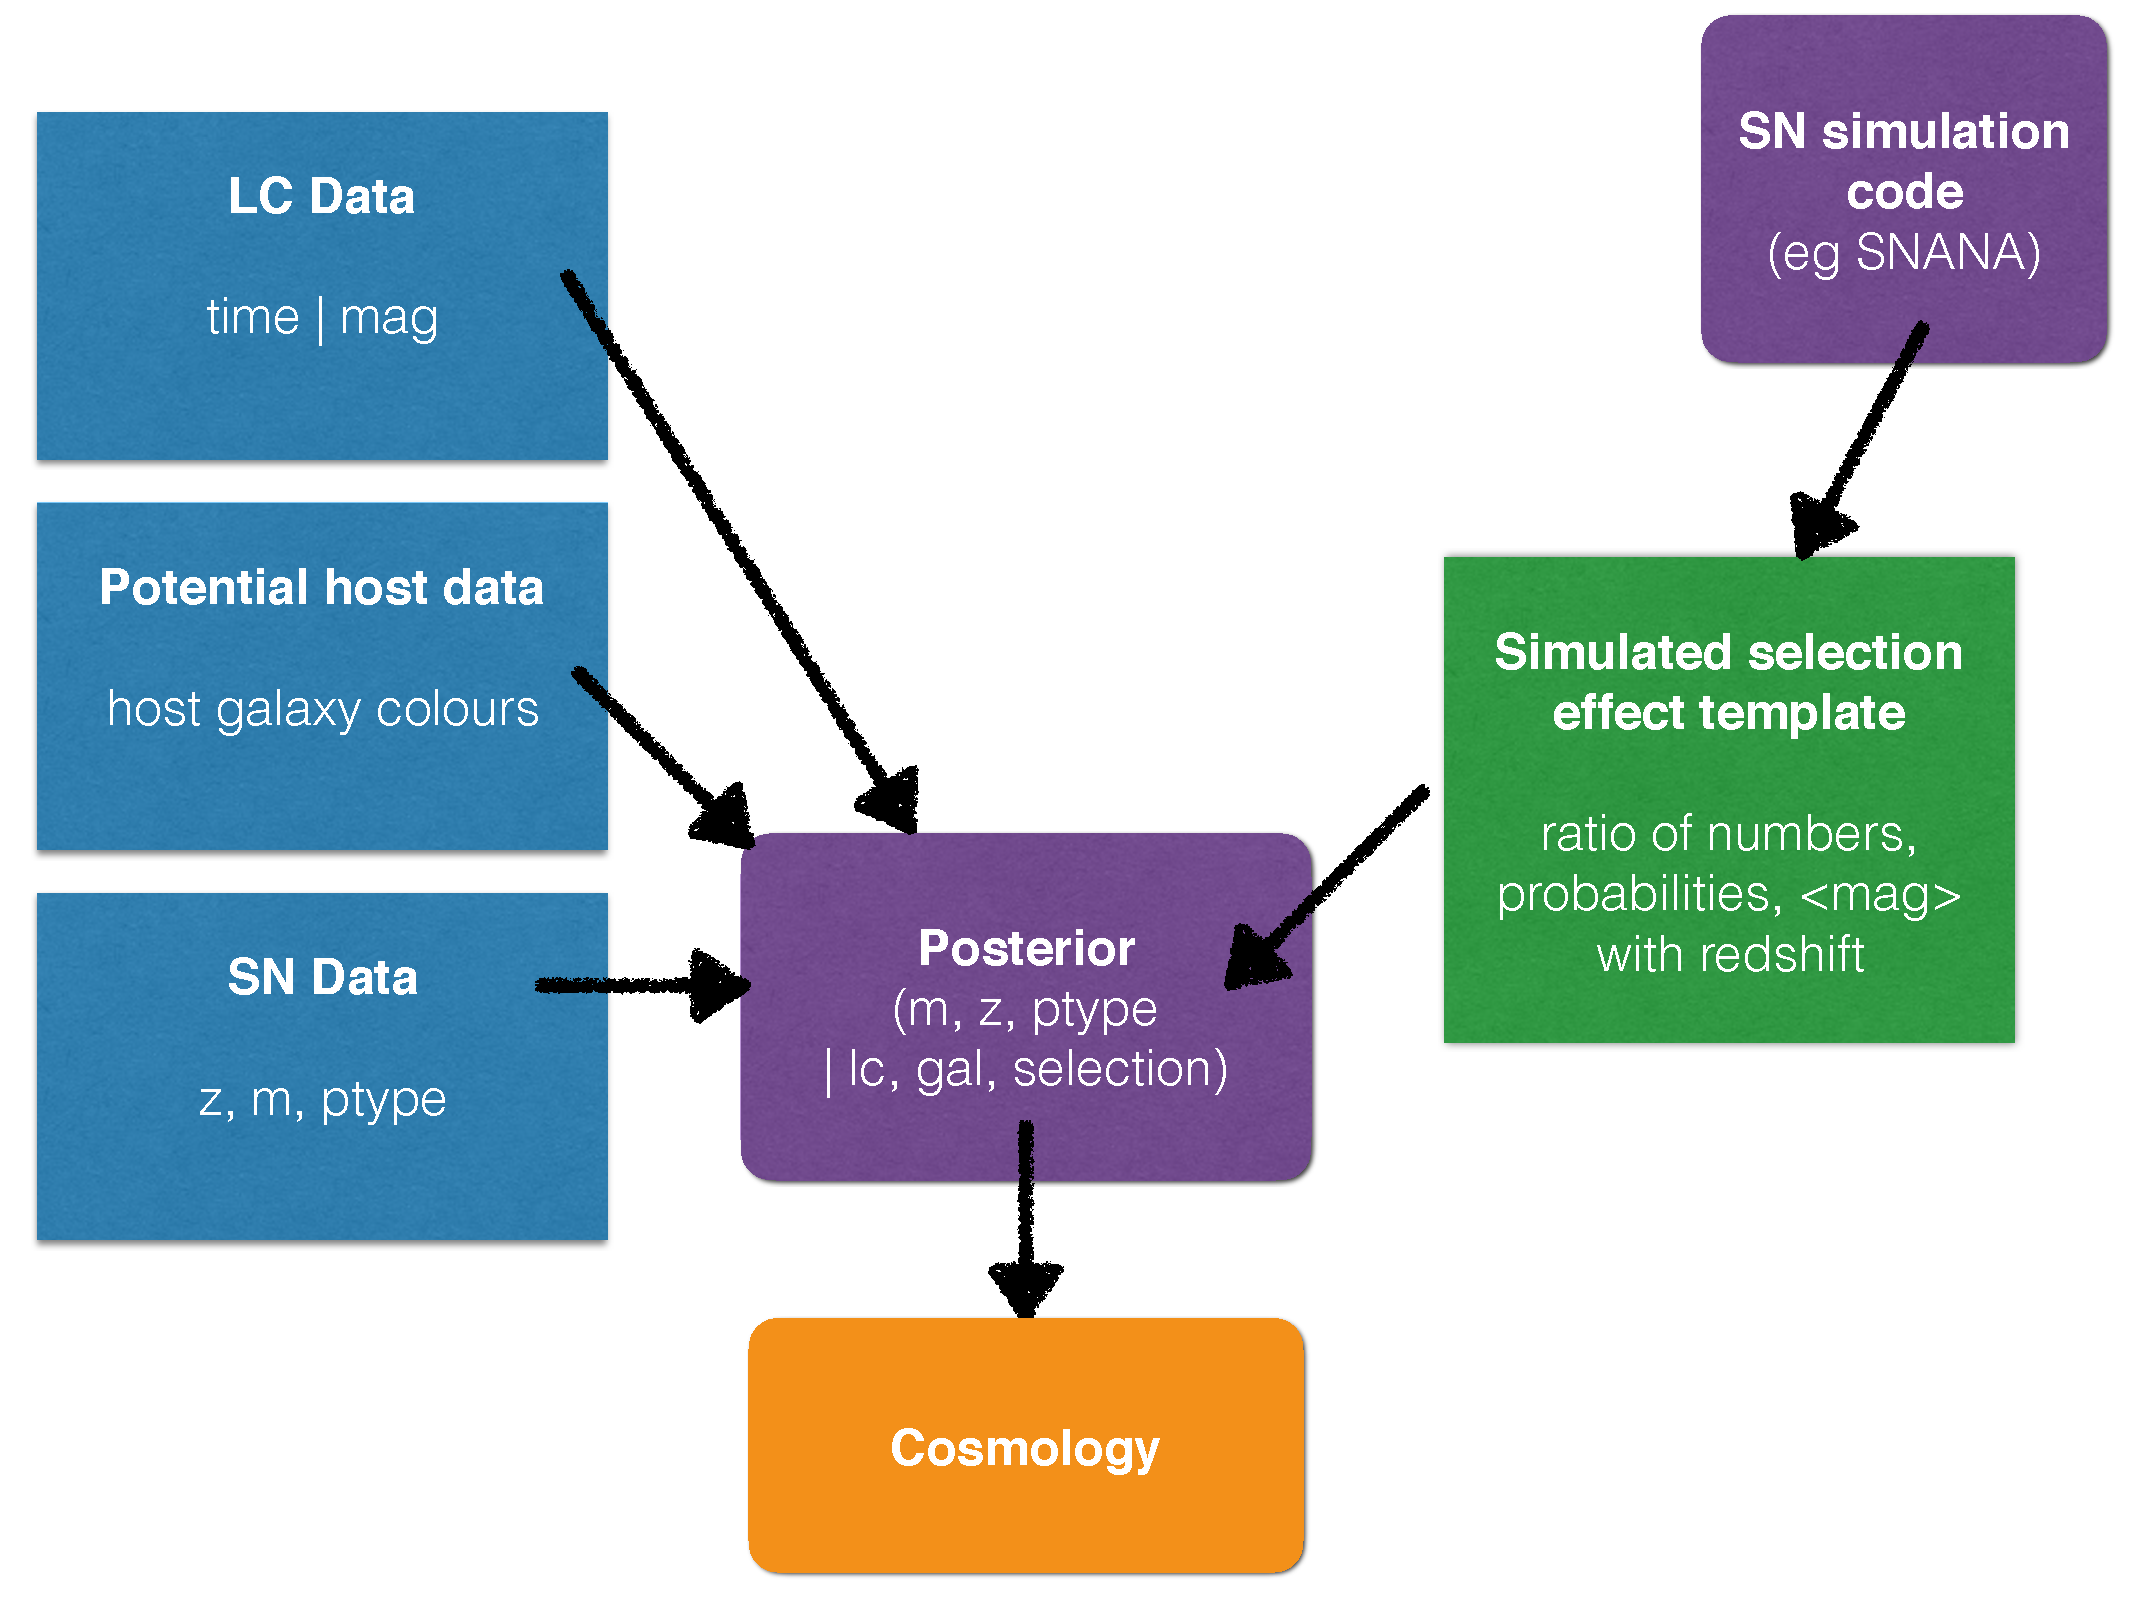
\includegraphics[width=1.0\textwidth]{fig/Schematic_Hlozek.pdf}\\
% \begin{tikzpicture}[node distance=1cm]

% \tikzstyle{data} = [rectangle, text centered, draw=black, fill=blue!20]
% \tikzstyle{prior} = [rectangle, text centered, draw=black, fill=red!20]
% \tikzstyle{selection} = [rectangle, text centered, draw=black, fill=green!20]
% \tikzstyle{posterior} = [rectangle, text centered, draw=black, fill=black!20]

% \node (nz) [hyper] {$N(z)$};
% \node (z) [param, below of=nz,yshift=-0.25cm] {$z_{j}$};
% \node (mags) [data, below of=z,yshift=-0.25cm] {$\vec{d}_{j}$};
% \node (survey) [draw=black,fit={(mags.west)(z.north)(mags.south)(mags.east)}] 
% {};
% \node [xshift=1.75cm,yshift=0.25cm] at (survey.south) {$j=1,\dots,J$};

% \draw [arrow] (nz) -- (z);
% \draw [arrow] (z) -- (mags);

% \end{tikzpicture}
\caption{{\bf The flow of the \scippr process:} by combining a prior-based selection function that is simulated for a given survey with the SN magnitudes, redshift and type and the potential host galaxy colours, the full posterior across both magnitude, type and galaxy properties is obtained 
\label{fig:flow1}}
\end{center}
\end{figure*}

\textbf{(@aimalz Discuss interim priors and selection functions in more detail here, or somewhere else?)}

The goal here is to constrain the posterior distribution $p(\vec{\Omega}, \textul{\phi} | \{\textul{\ell}_{n}\}_{N}, \{\vec{f}_{n}\}_{N})$ of the physically important hyperparameters in $\vec{\Omega}$ and $\textul{\phi}$ given a catalog of $N$ interim posterior distributions $p(t_{n}, z_{n}, \mu_{n} | \textul{\ell}_{n}, \textul{\xi}, \vec{\alpha})$ and another $N$ interim posterior distributions $p(z_{n} | \vec{f}_{n}, \vec{\theta}, \vec{\beta})$.  

The end goal is to derive an expression for the \textit{posterior distribution} over hyperparameters in terms of the interim posteriors over latent parameters.

We begin by expanding this in terms of Bayes' Rule:
\begin{align}
\label{eq:bayes}
p(\vec{\Omega}, \textul{\phi} | \{\textul{\ell}_{n}\}_{N}, \{\vec{f}_{n}\}_{N}) &\propto p(\vec{\Omega}, \textul{\phi})\ p(\{\textul{\ell}_{n}\}_{N}, \{\vec{f}_{n}\}_{N} | \vec{\Omega}, \textul{\phi})
\end{align}

The \textit{posterior probability} of a certain cosmology and redshift-dependent type proportions given some set of observed supernova lightcurves and host galaxy photometry is proportional to the product the prior on the cosomological parameters; the redshift-dependent type proportions and the likelihood of the lightcurves and host galaxy photometry \textit{given} the cosmology and redshift-dependent type proportions.

A key assumption is the statistical independence of the supernova parameters and observations; each set of $(t_{n'}, z_{n'}, \mu_{n'}, \textul{\ell}_{n'}, \vec{f}_{n'})$ is independent from all other parameters in $\bigcup_{n}(t_{n\neq n'}, z_{n\neq n'}, \mu_{n\neq n'}, \textul{\ell}_{n\neq n'}, \vec{f}_{n\neq n'})$.
\begin{align}
\label{eq:independence}
p(\{\textul{\ell}_{n}\}_{N}, \{\vec{f}_{n}\}_{N} | \vec{\Omega}, \textul{\phi}) &= \prod_{n}^{N}p(\textul{\ell}_{n}, \vec{f}_{n} | \vec{\Omega}, \textul{\phi})
\end{align}

This assumption is necessary for us to easily combine the contributions of individual supernovae to the likelihood of the whole survey of supernovae. Here we are saying the the likelihood of the set of lightcurves and fluxes is simply the product of each of the individual likelihoods.


We give the full derivation of the posterior in Appendix~\ref{appendix:derivation}, the final posterior on the cosmological parameters of interest and redshift-dependent type proportions is given as:

\begin{eqnarray}
\label{eq:wrapupmain}
p(\vec{\Omega}, \textul{\phi} | \{\textul{\ell}_{n}, \vec{f}_{n}\}_{N}) &\propto& p(\vec{\Omega}, \textul{\phi})\nonumber \\ &&\prod_{n}^{N}\ \iiint p(\mu_{n}, z_{n}, t_{n} | \textul{\ell}_{n}, \vec{f}_{n}, \vec{\theta}, \textul{\xi}, \vec{\alpha}, \vec{\beta}) \times \nonumber \\ &&\frac{p(\mu_{n}, z_{n}, t_{n} | \vec{\Omega}, \textul{\phi})}{p(\mu_{n}, z_{n}, t_{n} | \vec{\theta}, \textul{\xi}, \vec{\alpha}, \vec{\beta})}\ d\mu_{n}\ dz_{n}\ dt_{n},
\end{eqnarray}




It is very important to document the assumptions we make with this model:
\begin{enumerate}
	\item\label{it:completeness} The expression of Eq. \ref{eq:wrapupmain} is only as correct as the probabilistic graphical model of Fig. \ref{fig:pgm} is complete.
	\item\label{it:prior} We must choose a prior probability distribution $p(\vec{\Omega}, \textul{\phi})$.
	\item\label{it:interimpriors} The interim prior parameters $\vec{\theta}$ and $\textul{\xi}$ are known and shared among all supernovae and host galaxies $n$.
	\item\label{it:selectionfunctions} The selection function parameters $\vec{\beta}$ and $\textul{\alpha}$ are known and shared among all supernovae and host galaxies $n$.
	\item\label{it:independence} All latent and observed parameters associated with the supernovae and their host galaxies are statistically independent from the latent and observed parameters of all other supernovae and their host galaxies.
	\item\label{it:accuracy} The interim posterior distributions $\{p(z_{n} | \vec{f}_{n}, \vec{\theta}, \vec{\beta})\}_{N}$ and $\{p(t_{n}, z_{n}, \mu_{n} | \textul{\ell}_{n}, \textul{\xi}, \vec{\alpha})\}_{N}$ are accurate.
\end{enumerate}
There are a few caveats to these assumptions.  

Item \ref{it:completeness} is present with any approach, as no model can include every aspect of the physics -- to make any problem tractable, we must make simplifications.  The hierarchical Bayesian approach, however, easily accommodates complications so is extensible to more refined models.

Skeptics of Bayesian statistics often cite item \ref{it:prior} as a major weakness of this approach.  It is true that choosing a prior distribution can impart a bias on the resulting inference, but it can be an advantage when the data quality is poor and there are already trustworthy constraints on the parameters in question.  We will nonetheless try to minimize the information imparted to the posterior by the prior.

It is noted that this model may be adapted to the cases when Items \ref{it:interimpriors} and \ref{it:selectionfunctions} are violated, which will be the case if the interim posteriors are not derived by a single method or if the photometry comes from a combination of surveys.  

Item \ref{it:independence} is never truly valid in that all data observed by a single instrument are correlated, for example, but if the data primarily inform us about the phenomenon in question and we believe the principle of the universality of physics, it is a safe assumption; furthermore, virtually no statistical analysis would be possible without it, so all alternative methods already make this assumption.

It may seem to go without saying, but Item \ref{it:accuracy} can be difficult to guarantee.  As will be discussed further in Sec. \ref{sec:data}, there is as yet no established method for producing the interim posterior distributions, and validating any such method's accuracy will be a challenge, as it has proven to be for photo-$z$ PDFs.

We implement the model of Sec. \ref{sec:model} in the form of the Supernova Cosmology Inference with Probabilistic Photometric Redshifts code \scippr, which is a \texttt{Python} code freely available to the community.

\section{Mock Data}
\label{sec:data}

The mock data used to validate this method is unusual in that joint interim posteriors over supernova type, redshift, and distance modulus have never before been made.  This paper does not approach the problem of how to produce this data product because doing so would require us to make many more assumptions that could limit the impact of this work.  As was mentioned in Sec. \ref{sec:model}, it is nontrivial to confirm the accuracy of any probabilistic data analysis method.  Doing so will require painstaking simulations of lightcurves and host galaxy photometry as well as a choice of lightcurve fitting scheme, a sufficiently complex endeavor to leave for future work.  

Instead of simulating supernova lightcurves and host photometry, we take the true values of parameters of supernova type, redshift, and distance modulus to be proxies for the lightcurves and host galaxy photometry.  The data product in hand is a catalog of three-dimensional post-selection interim posteriors constructed according to the forward model of Figure \ref{fig:simflow}, which will be described in detail in the following sections.

\begin{figure*}
\vspace{0.5cm}
\begin{center}
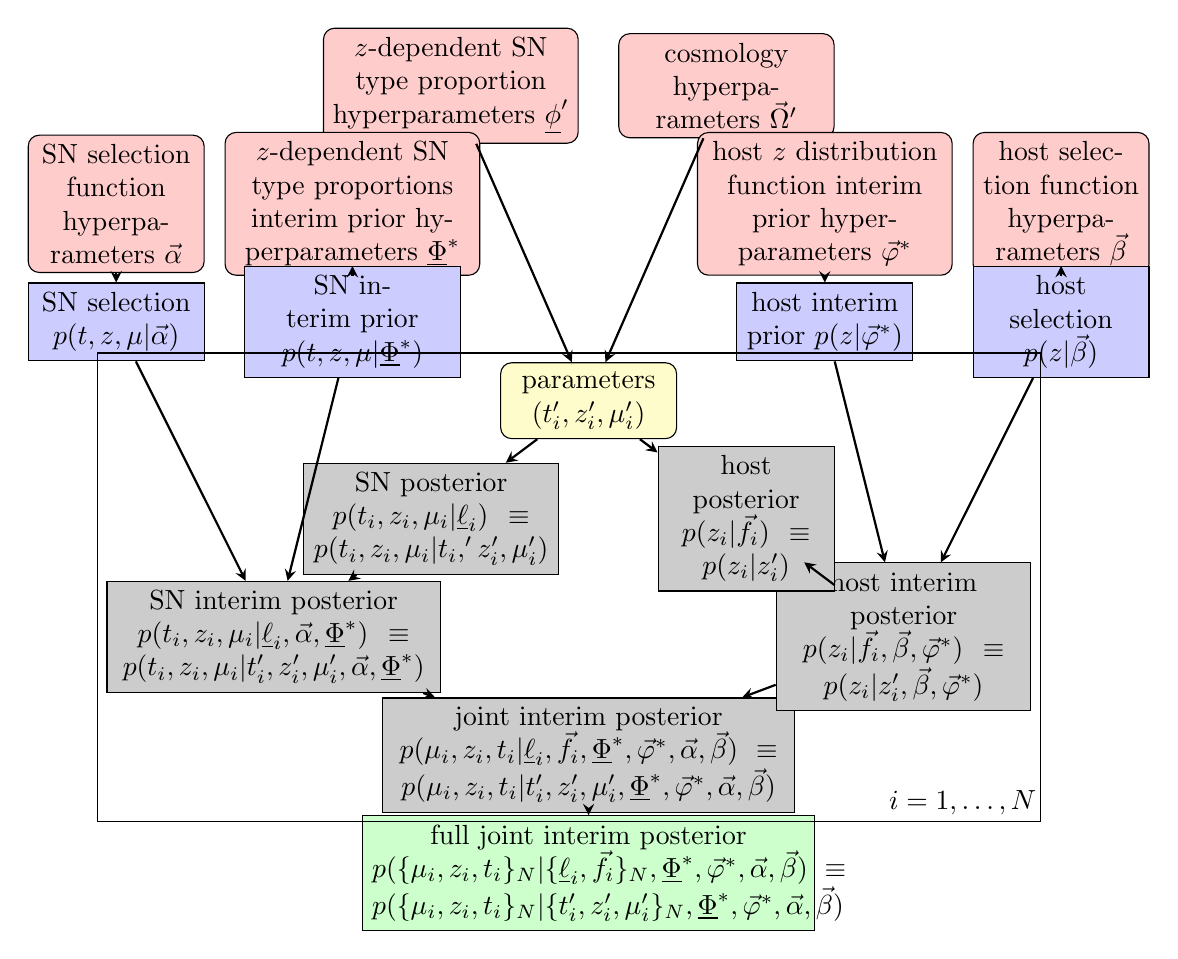
\begin{tikzpicture}[node distance=1cm]

\node (joint) [full, text width=5cm] {joint interim posterior $p(\mu_{i}, z_{i}, t_{i} | \textul{\ell}_{i}, \vec{f}_{i}, \textul{\Phi}^{*}, \vec{\varphi}^{*}, \vec{\alpha}, \vec{\beta})\ \equiv\ p(\mu_{i}, z_{i}, t_{i} | t'_{i}, z'_{i}, \mu'_{i}, \textul{\Phi}^{*}, \vec{\varphi}^{*}, \vec{\alpha}, \vec{\beta})$};

\node (fulljoint) [final, below of=joint, text width=5.5cm, yshift=-0.5cm] {full joint interim posterior $p(\{\mu_{i}, z_{i}, t_{i}\}_{N} | \{\textul{\ell}_{i}, \vec{f}_{i}\}_{N}, \textul{\Phi}^{*}, \vec{\varphi}^{*}, \vec{\alpha}, \vec{\beta})\ \equiv\ p(\{\mu_{i}, z_{i}, t_{i}\}_{N} | \{t'_{i}, z'_{i}, \mu'_{i}\}_{N}, \textul{\Phi}^{*}, \vec{\varphi}^{*}, \vec{\alpha}, \vec{\beta})$};

\node (fullhost) [posterior, above of=joint, xshift=4.0cm, yshift=0.5cm, text width=3.0cm] {host interim posterior $p(z_{i} | \vec{f}_{i}, \vec{\beta}, \vec{\varphi}^{*})\ \equiv\ p(z_{i} | z_{i}', \vec{\beta}, \vec{\varphi}^{*})$};
\node (fullSN) [posterior, above of=joint, xshift=-4.0cm, yshift=0.5cm, text width=4.0cm] {SN interim posterior $p(t_{i}, z_{i}, \mu_{i} | \textul{\ell}_{i}, \vec{\alpha}, \textul{\Phi}^{*})\ \equiv\ p(t_{i}, z_{i}, \mu_{i} | t_{i}', z_{i}', \mu_{i}', \vec{\alpha}, \textul{\Phi}^{*})$};

\node (hostpost) [data, above of=fullhost, xshift=-2.0cm, yshift=0.5cm, text width=2.0cm] {host posterior $p(z_{i} | \vec{f}_{i})\ \equiv\ p(z_{i} | z'_{i})$};
\node (SNpost) [data, above of=fullSN, xshift=2.0cm, yshift=0.5cm, text width=3.0cm] {SN posterior $p(t_{i}, z_{i}, \mu_{i} | \textul{\ell}_{i})\ \equiv\ p(t_{i}, z_{i}, \mu_{i} | t_{i},' z_{i}', \mu_{i}')$};

\node (trueparams) [params, above of=joint, yshift=3.5cm, text width=2.0cm] {parameters $(t'_{i}, z'_{i}, \mu'_{i})$};

\node (truecosmo) [model, above of=trueparams, xshift=1.75cm, yshift=3.0cm, text width=2.5cm] {cosmology hyperparameters $\vec{\Omega}'$};
\node (trueprops) [model, above of=trueparams, xshift=-1.75cm, yshift=3.0cm, text width=3.0cm] {$z$-dependent SN type proportion hyperparameters $\textul{\phi}'$};

\node (SNintprparam) [model, above of=trueparams, xshift=-3.0cm, yshift=1.5cm, text width=3.0cm] {$z$-dependent SN type proportions interim prior hyperparameters $\textul{\Phi}^{*}$};
\node (hostintprparam) [model, above of=trueparams, xshift=3.0cm, yshift=1.5cm, text width=3.0cm] {host $z$ distribution function interim prior hyperparameters $\vec{\varphi}^{*}$};

\node (hostintpr) [prior, below of=hostintprparam, yshift=-0.5cm, text width=2.0cm] {host interim prior $p(z | \vec{\varphi}^{*})$};
\node (SNintpr) [prior, below of=SNintprparam, yshift=-0.5cm, text width=2.5cm] {SN interim prior $p(t, z, \mu | \textul{\Phi}^{*})$};

\node (SNselfunparam) [model, above of=trueparams, xshift=-6.0cm, yshift=1.5cm, text width=2.0cm] {SN selection function hyperparameters $\vec{\alpha}$};
\node (hostselfunparam) [model, above of=trueparams, xshift=6.0cm, yshift=1.5cm, text width=2.0cm] {host selection function hyperparameters $\vec{\beta}$};

\node (hostselfun) [selection, below of=hostselfunparam, yshift=-0.5cm, text width=2.0cm] {host selection $p(z | \vec{\beta})$};
\node (SNselfun) [selection, below of=SNselfunparam, yshift=-0.5cm, text width=2.0cm] {SN selection $p(t, z, \mu | \vec{\alpha})$};

\node (survey) [draw=black,  fit=(fullSN.west)(trueparams.north)(joint.south)(fullhost.east)] 
{};
\node [xshift=5.0cm,yshift=0.25cm] at (survey.south) {$i=1,\dots,N$};

\draw [arrow] (fullhost) -- (joint);
\draw [arrow] (fullSN) -- (joint);
\draw [arrow] (hostselfunparam) -- (hostselfun);
\draw [arrow] (hostselfun) -- (fullhost);
\draw [arrow] (hostintprparam) -- (hostintpr);
\draw [arrow] (hostintpr) -- (fullhost);
\draw [arrow] (hostpost) -- (fullhost);
\draw [arrow] (SNselfunparam) -- (SNselfun);
\draw [arrow] (SNselfun) -- (fullSN);
\draw [arrow] (SNintprparam) -- (SNintpr);
\draw [arrow] (SNintpr) -- (fullSN);
\draw [arrow] (SNpost) -- (fullSN);
\draw [arrow] (truecosmo) -- (trueparams);
\draw [arrow] (trueprops) -- (trueparams);
\draw [arrow] (trueparams) -- (hostpost);
\draw [arrow] (trueparams) -- (SNpost);
\draw [arrow] (joint) -- (fulljoint);

\end{tikzpicture}
\caption{An illustration of the mock data generation procedure.  Red boxes represent hyperparameter values we choose for realism; blue boxes represent a priori probability distributions shared by all observed objects; yellow boxes represent parameter values unique to each object; gray boxes represent probability distributions unique to each object; green boxes represent the probability distributions derived from all information in the survey.}
\label{fig:simflow}
\end{center}
\end{figure*}

In this section, we outline the forward model by which the mock interim posteriors are generated.  

\subsection{The true hyperparameters and parameters}
\label{sec:true_hypers}

We begin by choosing parametrizations for the hyperparameters.  We must have some functions of the hyperparameters producing a distribution from which the supernova type, redshift, and distance modulus are drawn.  Sections \ref{sec:TypeIaRate, sec:TypeIbcRate, sec:TypeIIRate} outline the model for realistic hyperparameters $\textul{\phi}$, with an overall model and the resulting redshift-dependent supernova type proportions illustrated in Table \ref{tab:sntypes} and Figure \ref{fig:srelative_supernova_rates} respectively.  Section \ref{sec:cosmohypers} provides the cosmological parameters used.  In Section \ref{sec:drawmock}, we show the results of drawing the true types, redshifts, and distance moduli from this model.

% \subsubsection{Redshift-dependent supernova type proportions}
% \label{sec:sntypes}

\begin{deluxetable*}{|p{4cm}|p{5cm}| c |p{5cm} |}
	\tabletypesize{\small}
	\tablecolumns{4}
	\tablecaption{Simulated Data Generation \label{tab:SimualtedDataGeneration}}
	\tablehead{\colhead{ } & \colhead{Ia} & \colhead{Ibc} & \colhead{II}}
	\startdata
	true cosmology hyperparameters & \multicolumn{3}{c}{\cite{Planck2014}} \\ \hline
	redshift dependent type proportions & \multicolumn{3}{c}{$p(t,z | \phi)$} \\ \hline
	number of SNe per volume per redshift & $\Psi$: delay time distribution &  ? & $K_{II}$: fraction of stars that explode as SNII \citep{Salpeter1955} \\ 
	{} & $SFH$: cosmic star formation history &  ? & $SFR$: Star formation rate (\citealt{Cole2001}, \citealt{Horiuchi2011}, \citealt{Madau2014}) \\
	{} & $R_{Ia}$ = $\Psi$ x $SFH$ &  ? & $R_{II}$ = $K_{II}$ x $SFR$ \\ \hline
	spectral models as a function of time & SN Ia 1994D &  ? & CSP-like SNe II simulated using MCMC \\ \hline
	K-corrections between bands & \cite{Hsiao2007} &  ? & \cite{Dessart2013} \\ \hline
	LSST filter throughputs & \multicolumn{3}{c}{\parbox[c]{10cm}{SysEng-approved LSST throughput curves \\ github.com/lsst/throughputs/tree/master/baseline}} \\ \hline
	LSST single epoch limiting magnitudes & \multicolumn{3}{c}{\parbox[c]{10cm}{\cite{LSSTScienceBook} \\ $u$=23.60 $g$=24.83 $r$=24.38 $i$=23.92 $z$=23.35}} \\ \hline
	Classified types of detected lightcurves & ? & ? & ? \\ \hline
	\enddata
\end{deluxetable*}

\vspace{1cm}

For the redshift-dependent type proportions, we choose $p(t, z | \textul{\phi})$ to be a two-dimensional piecewise constant function over $T$ types and $Z$ redshift bins, making $\textul{\phi}$ a $T\times Z$ array with values $\phi_{i}$ equal to the probability of a supernova having the given type with a redshift in a given bin.  A normalization condition is enforced such that summing over the discrete variable of supernova type and integrating over all redshift bins yields a value of unity.  

To demonstrate that \scippr is an extension of BEAMS, we consider $T=3$, with $\tau\in\{Ia, Ibc, II\}$.  Under this parametrization, we use realistic values for the elements of $\textul{\phi}'$ derived by convolving the delay time distribution (DTD) and the star formation history.  This procedure is outlined in Secs. \ref{sec:TypeIaRate}, \ref{sec:TypeIbcRate}, and \ref{sec:TypeIIRate}.  As an overview, we set the relative rates of SN Ia and Core Collapse to be 25\% and 75\%, respectively, at z = 0.  \textbf{(@tinapeters How were these numbers modified for three SN populations?)}  We use the DTD for SN Ia from Graur et al (2013) and the DTD for SN II from Zapartas et al (2017), and the Cosmic Star Formation Rate from Behroozi et al (2013).  \textbf{(@tinapeters Put these references into the .bib file.)}  The redshift-dependent supernova type proportions derived in this way are shown in Fig. \ref{fig:relative_supernova_rates}.  \textbf{(@tinapeters What is the native format of these curves, i.e. a continuous function evaluated on a grid or something else?  I wrote about a piecewise constant function, but it can and should be whatever's consistent with the actual functions you calculated.)}  $N=10^{4}$ pairs of $(t'_{n}, z'_{n})$ are drawn from this distribution.

\begin{figure}
	\begin{center}
		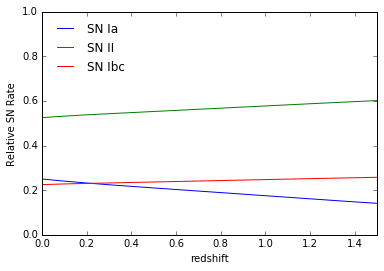
\includegraphics[width=0.5\textwidth]{fig/relative_supernova_rate.png}
		\caption{The relative supernova rates as a function of redshift. Sums to one at every redshift (but should actually integrate to one over type and redshift).  \textbf{(@aimalz Also plot the "observed" version of this for our sample)}}
		\label{fig:relative_supernova_rates}
	\end{center}
\end{figure}

\subsubsection{Supernova Type Ia Rate with Redshift}
\label{sec:TypeIaRate}

\subsubsection{Supernova Type Ibc Rate with Redshift}
\label{sec:TypeIbcRate}

\subsubsection{Supernova Type II Rate with Redshift}
\label{sec:TypeIIRate}

To determine the rate of SNII per unit comoving volume we will basically apply the approach by Forster et al. 2006/Strogler et al. 2004 adapted to SNe II following Botticella et al. 2012.

The rate of SNe II per unit time per unit comoving volume ($R_{II}$) is given by the star formation rate ($SFR$) per unit time per unit comoving volume convolved with the number of stars crearted that will explode as SNe II.

\begin{align}
	\label{eq:rateII_1}
	R_{II} = K_{II} \times SFR
\end{align}

First, we must calculate the fraction of stars that explode as SN II:

\begin{align}
\label{eq:rateII_2}
K_{II} = \frac{\int_{m_{l,II}}^{m_{u,II}} \phi(m) \mathrm{d}m}{\int_{m_{l}}^{m_{u}} m\phi(m) \mathrm{d}m}
\end{align}

When we integrate from a minimum mass, $m_{l,II}$, of 8 to a maximum mass, $m_{u,II}$, to 25 and assuming a Salpeter et al. (1955) IMF we get a rate of $6.027 \time 10^{-3}$.

We will use three different models of how the SFR evolutions with redshift: Cole et al. (2001), Horiuchi et al. (2011), and Madau et al. (2014)

\begin{figure}
	\begin{center}
		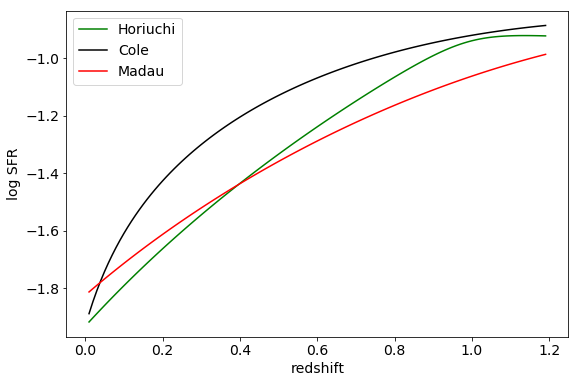
\includegraphics[width=0.5\textwidth]{fig/SNII_SFR.png}
		\caption{SFR evolutions with redshift: Cole et al. (2001), Horiuchi et al. (2011), and Madau et al. (2014).}
		\label{fig:SNII_SFR}
	\end{center}
\end{figure}

Next we will take the spectral model of Dessart et al. (2013) which is anchored to SN II 1999em, as a reference. We simulate its $r$-band light curve at different redshifts and convolve it with the LSST filters to see when it falls below the detection limit.

\begin{figure}
	\begin{center}
		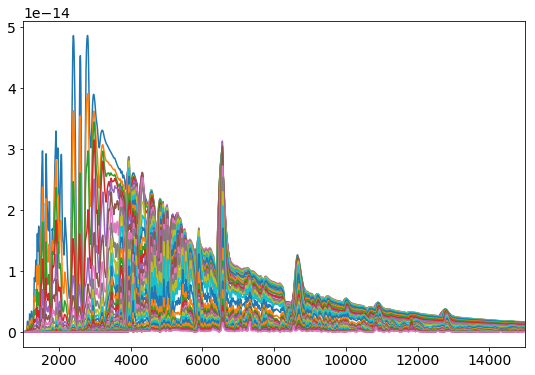
\includegraphics[width=0.5\textwidth]{fig/spectral_model_SNII.png}
		\caption{SN II spectral model of Dessart et al. (2013): $M_{99em}=-16.6$; $M_{05J}=-17.2$}
		\label{fig:SNII_lc}
	\end{center}
\end{figure}

\begin{figure}
	\begin{center}
		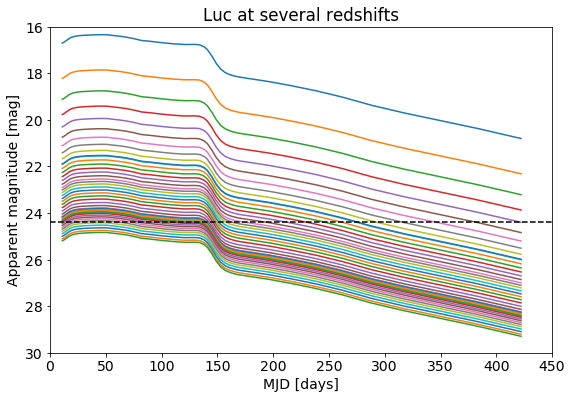
\includegraphics[width=0.5\textwidth]{fig/SNII_lc_withz.png}
		\caption{The $r$-band lightcurve of spectral model of SN II 1999em shifted to a range of redshifts. The horizontal dashed line indicates the limiting magnitude of LSST in the $r$-band in a single visit.}
		\label{fig:SNII_lc_withz}
	\end{center}
\end{figure}

For this model SN II, we compare the magnitude as a function of time and redshift, $m(t,z)$, with the limiting magnitude, $m_{lim}$, of the LSST camera to obtain the probability of detecting (the peak of) a SN at a given redshift, $\Delta_{t}(z)$. Then we estimate the number of detected SNe II per unit of redshift, $dN/dz$, using Equations 2 and 5 of Forster et al. (2006).

\begin{figure}
	\begin{center}
		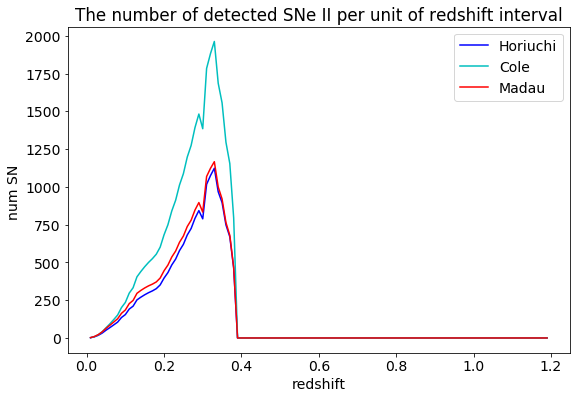
\includegraphics[width=0.5\textwidth]{fig/number_SNII.png}
		\caption{The number of SN II detected, for each of the SFR models, as a function of redshift. The total number of SN II for Horiuchi et al. 16985, Cole et al. 29207, and Madau et al.  18322. }
		\label{fig:SNII_lc_sfr}
	\end{center}
\end{figure}

Finally, we will use a a sample of 10,000 SNe, simulated using MCMC on real parameters of CSP SNe II. We will put each at 100 random redshifts from 0.01 to 1.20, so we will have 1,000,000 SNe. Now we consider the magnitude at the end of the plateau phase, instead of the peak magnitude. This is because in SN II cosmology, we do not standardize the magnitude at peak, but either the magnitude at around the center of the plateau (for spectroscopic methods), or the length/brightness-decline of the plateau (for photometric methods).

We use the apparent magnitudes at the end of the plateau phase and k-correct the magnitudes. Then we measure $\Delta_t(z)$, selecting different magnitude limit depending on the filter we use for observations. Finally, we compare the number of supernovae as a function of redshift for the three different SFR models.

\begin{figure}
	\begin{center}
		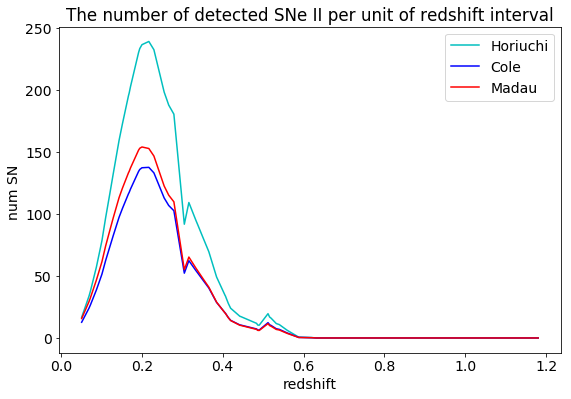
\includegraphics[width=0.5\textwidth]{fig/number_SNII_withmagntiudescatter.png}
		\caption{The number of SN II detected, for each of the SFR models, as a function of redshift. The total number of SN II for Horiuchi et al. 16985, Cole et al. 29207, and Madau et al.  18322. }
		\label{fig:SNII_lc_wz}
	\end{center}
\end{figure}

\subsubsection{Cosmological parameters}
\label{sec:cosmohypers}

For the parametrization of the cosmological parameters, we assume a $\Lambda$CDM cosmology so $\vec{\Omega}$ is comprised of $H_{0}$, $\Omega_{m}$, etc.  We choose the true cosmological parameters comprising $\vec{\Omega}'$ to be the maximum likelihood point estimates observed by Planck: $H_{0}=67.9\ Mpc/km/s$ and $\Omega_{m}=0.307$.  \textbf{(@aimalz fix these constants here and in code)}  The function that produces $\mu$ from a given $z_{n}$ is 
\begin{align}
\label{eq:distmod}
\mu &= 5\log\left[(1+z)\frac{1}{10\ pc}\int_{0}^{z}\frac{dz'}{\sqrt{\Omega_{M}(1+z)^{3}+\Omega_{k}(1+z)^{2}+\Omega_{\Lambda}}}\right].
\end{align}
This means that once the pair $(t'_{n}, z'_{n})$ is drawn from $p(t, z | \textul{\phi}')$, $p(\mu_{n} | \vec{\Omega}', z')$ is a delta function centered at $\mu'_{n}$ following Eq. \ref{eq:distmod}.  We have now set the true values of the hyperparameters and parameters

% $\textul{\phi}$ represents the parameters defining the supernova type proportions as a function of redshift, which we choose to be a $T\times Z$ dimensional matrix for a space with $T$ possible supernova types $\tau$ and $Z$ redshift bins $\zeta$ of widths $\vec{\Delta}_{z}$, where each element of $\phi_{\tau\zeta}$ is the probability density associated with a supernova of type $\tau$ with a redshift in bin $\zeta$; thus we have $p(z_{\zeta}, t_{\tau} | \textul{\phi}) \equiv \phi_{\zeta\tau}$, with $\textul{\phi}$ satisfying the normalization condition $\sum_{\tau=1}^{T}\textul{\phi}\cdot\vec{\Delta}_{z}=1$.  We proceed to choose a physically motivated true matrix of redshift-dependent supernova type proportions $\textul{\phi}'$.
 
\subsubsection{Setting true values of the latent variables}
\label{sec:drawmock}

To conclude Section \ref{sec:true_hypers}, we visualize the resulting true parameters $\{(t_{n}', z_{n}', \mu_{n}')\}_{N}$ in Figure \ref{fig:obs_rates}.  If we were able to plot all supernovae on a Hubble diagram, we would obtain Figure \ref{fig:true_hubble}.

\begin{figure}
	\begin{center}
		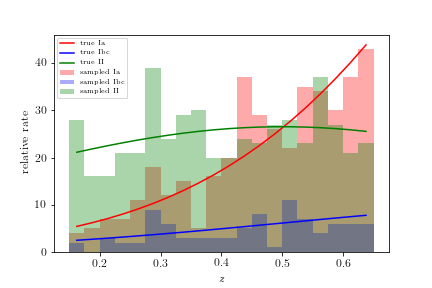
\includegraphics[width=0.5\textwidth]{fig/obs_rates.png}
		\caption{The true types and redshifts of $N=1000$ supernovae.}
		\label{fig:obs_rates}
	\end{center}
\end{figure}

\begin{figure}
	\begin{center}
		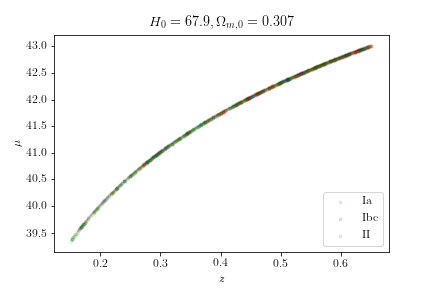
\includegraphics[width=0.5\textwidth]{fig/true_hubble.png}
		\caption{The Hubble diagram plotted as if all supernova types were standardizable and perfectly measured.}
		\label{fig:true_hubble}
	\end{center}
\end{figure}
%
% To review, the latent variables are the supernova types $\{t_{n}\}_{N}$, redshifts $\{z_{n}\}_{N}$, and distance moduli $\{\mu_{n}\}_{N}$.  Now we must set a parametrization on the probability distributions $p(\mu_{n}, z_{n}, t_{n} | \textul{\ell}_{n}, \vec{f}_{n})$.  For the supernova type and redshift dimensions, we adopt the same parametrization used for $\textul{\phi}$.  There are $T$ supernova types and $Z$ redshift bins, indexed by $\tau$ and $\zeta$ respectively/  W, and $D$ bins in distance modulus indexed by $\nu$.  $\textul{\phi}$ describes 
%
% Because the redshift-dependent supernova type proportions are parametrized by $\textul{\phi}'$ such that $p(z\in\zeta, t=\tau | \textul{\phi}') = \phi_{\zeta\tau}$, it is easy to draw pairs of true types and redshifts $(t_{n}', z_{n}')$ from $\textul{\phi}'$.  We treat the elements of $\textul{\phi}'$ as a discrete distribution, noting that the redshift-dependent supernova type proportions are normalized such that $\sum_{\tau}\int_{\zeta}\textul{\phi}=1$.  Sampling the function defined by $\textul{\phi}'$ is equivalent to sampling true types and redshift bins.  Once the redshift bins have been chosen, we may choose a true redshift for each supernova from a uniform distribution defined between the bin endpoints.  This procedure gives us pairs of true types and redshifts $(t_{n}', z_{n}')$.
%
% Finally, we calculate the true $\mu_{n}'$ according to [insert distance modulus equation from astropy.cosmology here] from $z_{n}'$ and $\vec{\theta}'$.  Rather than writing the form of the distance modulus as a function of redshift and cosmological parameters throughout the paper, we will instead use the shorthand $\mu = f_{\vec{\theta}}(z)$ here.  This results in a true catalog of length $N$ consisting of trios $(t_{n}', z_{n}', \mu_{n}')$ of the latent variables.

\subsection{Supernova lightcurve-based PDFs}
\label{sec:snlcpdf}

Each supernova in the sample must have a three-dimensional probability distribution, which will be an interim posterior, over the type, redshift, and distance modulus, combined as
\begin{align}
    \label{eq:fullsnlcpdf}
    p(t, z, \mu | \textul{\ell}_{i}, \vec{\alpha}, \textul{\Phi}^{*}) = p(t, z, \mu | t_{i}', z_{i}', \mu_{i}', \vec{\alpha}, \textul{\Phi}^{*}) &= p(t, z, \mu | t_{i}', z_{i}', \mu_{i}')\ p(t, z, \mu | \textul{\Phi}^{*})] p(t, z, \mu | \vec{\alpha}),
\end{align}
or, in words
\begin{equation}
    \label{eq:fullsnlcpdfwords}
    [\textrm{supernova post-selection interim posterior}]_{i} = [\textrm{lightcurve posterior}]_{i}\ \boldsymbol{\cdot}\ \textrm{type-redshift-distance modulus interim prior}\ \boldsymbol{\cdot}\ \textrm{supernova selection function}.
\end{equation}
Sections \ref{sec:snlcposterior, sec:snlcinterim, sec:snlcselection} cover the production of the lightcurve posteriors, the type-redshift-distance modulus interim prior, and supernova selection function respectively.

\subsubsection{Supernova lightcurve data model}
\label{sec:snlcposterior}

We present our model for emulating three-dimensional posteriors $p(t, z, \mu | \textul{\ell}_{i})\equiv p(t, z, \mu | t_{i}', z_{i}', \mu_{i}')$.  In current analyses, supernovae are classified before the lightcurve is fit, so we first emulate $p(t | t_{i}')$ using a typical confusion matrix of an unspecified classifier.  The confusion matrix, illustrated in Table \ref{tab:confusionmatrix} has elements of $p(t', \hat{t})$, where $t'$ is the true type of a supernova and $\hat{t}$ is the classified type.  We note that the confusion matrix satisfies a normalization condition $\sum_{t'}\sum{\hat{t}}p(t', \hat{t})=1$.  By invoking Bayes' Rule, we can derive the desired classification probabilities $p(\hat{t} | t')=p(t', \hat{t})/p(t')$.  We know $p(t')$ for our mock data because we set $\textul{\phi}'$, and the confusion matrix provides $p(t', t)=p(t', \hat{t})$.  In reality, not all supernovae of a single true type will have the same type posterior $p(t | \textul{\ell}_{i})$, but we make use of this simplification for now because we do not know enough about the output of a fully probabilistic lightcurve classifier to make a more realistic model.  For these purposes we use the confusion matrix of\dots \textbf{(Choose a particular classifier's confusion matrix!)}

% \vspace{1in}
% \begin{figure}
% \renewcommand\arraystretch{1.5}
% \setlength\tabcolsep{0pt}
\begin{tabular}{l @{\hspace{0.7em}}r @{\hspace{0.7em}}c @{\hspace{0.4em}}c @{\hspace{0.4em}}c @{\hspace{0.7em}}l}
    \multirow{17}{*}{\rotatebox{90}{\parbox{3.0cm}{\bfseries\centering Simulation Input}}} & & \multicolumn{3}{c}{\bfseries Classification Output} &  \\
	 & & $\hat{t} = \RN{1}a$ & $\hat{t} = \RN{1}bc$ & $\hat{t} = \RN{2}$ & \bfseries total \\
	& \em{t' = \RN{1}a} & \MyBox{$p(t' = \RN{1}a, \hat{t} = \RN{1}a)$}{ \ } & \MyBox{$p(t' = \RN{1}a, \hat{t} = \RN{1}bc)$}{ \ } & \MyBox{$p(t' = \RN{1}a, \hat{t} = \RN{2})$}{ \ } & Simulated \RN{1}a Rate \\[2.4em]
	& \em{t' = \RN{1}bc} & \MyBox{$p(t' = \RN{1}bc, \hat{t} = \RN{1}a)$}{ \ } & \MyBox{$p(t' = \RN{1}bc, \hat{t} = \RN{1}bc)$}{ \ } & \MyBox{$p(t' = \RN{1}bc, \hat{t} = \RN{2})$}{ \ } & Simulated Ibc Rate\\[2.4em]
	& \em{t' = \RN{2}} & \MyBox{$p(t' = \RN{2}, \hat{t} = \RN{1}a)$}{ \ } & \MyBox{$p(t' = \RN{2}, \hat{t} = \RN{1}bc)$}{ \ } & \MyBox{$p(t' = \RN{2}, \hat{t} = \RN{2})$}{ \ } & Simulated II Rate \\
    & {\bfseries total} & Classified \RN{1}a rate & Classified Ibc rate & Classified II rate & \\
    \label{tab:confusionmatrix}
\end{tabular}
%\caption{}
% \label{fig:confusion}
% \end{figure}

Next, we emulate $p(z, \mu | t, t'_{i}, z'_{i}, \mu'_{i})$, the redshift and distance modulus probabilities fit to a lightcurve given its classification, a three-dimensional object defined over dimensions of supernova type, redshift, and distance modulus.  We know $p(z, \mu | t=\mathrm{Ia}, t'_{i}=\mathrm{Ia}, z'_{i}, \mu'_{i})$ from the output of successful lightcurve fits.  Here, we use a bivariate Gaussian distribution $\mathcal{N}([z_{i}''^{\ell}, \mu_{i}''^{\ell}], \Sigma_{Ia})$ with a covariance $\Sigma_{Ia}$ shared by the entire dataset and a mean of $[z_{i}''^{\ell}, \mu_{i}''^{\ell}]$ drawn from a bivariate Gaussian distribution $\mathcal{N}([z'_{i}, \mu'_{i}], \Sigma_{Ia})$ of the same covariance with a mean of $[z'_{i}, \mu'_{i}]$, the true redshift and distance modulus.  

Since only type Ia supernovae are standardizable candles, we note that $p(z, \mu | t\neq\mathrm{Ia}, t'_{i}, z'_{i}, \mu'_{i})$ ought to be flat in the $\mu$ dimension.  We also have some idea of what $p(z, \mu | t=\mathrm{Ia}, t'_{i}\neq\mathrm{Ia}, z'_{i}, \mu'_{i})$ should look like from contaminated Hubble diagrams.  \textbf{(Let's find one such plot!)}  For $t'_{i}=\mathrm{Ibc}$, we use a bivariate Gaussian distribution $\mathcal{N}([z_{i}''^{\ell}, \mu_{i}''^{\ell}], \Sigma_{Ibc})$ with a covariance $\Sigma_{Ibc}$ shared by the entire dataset and a mean of $[z_{i}''^{\ell}, \mu_{i}''^{\ell}]$ drawn from a bivariate Gaussian distribution $\mathcal{N}([z'_{i}, \mu'_{i}-\mu_{Ibc}], \Sigma_{Ibc})$ of the same covariance with a mean of $[z'_{i}, \mu'_{i}-\mu_{Ibc}]$, the true redshift and a distance modulus downshifted from the true distance modulus by a constant $\mu_{Ibc}$ shared across the entire dataset.    For $t'_{i}=\mathrm{II}$, we use a bivariate Gaussian distribution $\mathcal{N}([z_{i}''^{\ell}, \mu_{i}''^{\ell}], \Sigma_{II})$ with a covariance $\Sigma_{II}$ shared by the entire dataset and a mean of $[z_{i}''^{\ell}, \mu_{i}''^{\ell}]$ drawn from a bivariate Gaussian distribution $\mathcal{N}([z'_{i}, \mu_{II}], \Sigma_{II})$ of the same covariance with a mean of $[z'_{i}, \mu_{II}]$, the true redshift and a constant distance modulus $\mu_{II}$  shared across the entire dataset.  

Finally, we combine then terms as $p(t, z, \mu | \textul{\ell}_{i})\equiv p(t, z, \mu | t_{i}', z_{i}', \mu_{i}')=p(t | t'_{i})p(z, \mu | t'_{i}, z'_{i}, \mu'_{i})$

\subsubsection{Supernova type-redshift-distance modulus analysis model}
\label{sec:snlcinterim}

An interim prior $p(t, z, \mu | \textul{\Phi}^{*})$ may be the supernova type-redshift-distance modulus distribution observed in a previous survey (training set) in the case of a template-based (machine learning) method for deriving interim posteriors.  In our mock data, we choose an interim prior defined by hyperparameters $\textul{\Phi}^{*}$ that contains a perturbed version of the true redshift-dependent type proportion parameters $\textul{\phi}'$ representing an initial guess and anontrivial distribution in the space of distance modulus.  We take a the distance modulus from Equation \ref{eq:distmod} evaluated at interim prior cosmological parameters $\vec{\Omega}^{*}$ from WMAP, including its error bars to produce a broad distribution in the space of distance modulus.

\subsubsection{Supernova selection function}
\label{sec:snlcselection}

Though the selection function $p(\textul{\ell} | \vec{\alpha})$ for a survey occurs in the space of lightcurves $\textul{\ell}$, it is always projected into the space of lightcurve fit parameters.  We use a selection function $p(t, z, \mu | \vec{\alpha}$ that is flat with respect to the distance modulus but has nontrivial structure in the space of type and redshift.  Our empirical selection function is based on the ratio of the recovery rates of supernovae as a function of type and redshift in two simulated surveys, one representing a realistic observing strategy, LSST's wide-fast-deep (WFD) strategy, and one representing a best case observing strategy, LSST's deep drilling field (DDF) strategy,
\begin{equation}
    \label{eq:snlcselfunwords}
    p(t, z, \mu | \vec{\alpha}) = \frac{\frac{\mathrm{number\ of\ recovered\ type\ }t\mathrm{\ SNe\ at\ redshift\ }z\mathrm{\ in\ WFD}}{\mathrm{number\ of\ simulated\ type\ }t\mathrm{\ SNe\ at\ redshift\ }z\mathrm{\ in\ WFD}}}{\frac{\mathrm{number\ of\ recovered\ type\ }t\mathrm{\ SNe\ at\ redshift\ }z\mathrm{\ in\ DDF}}{\mathrm{number\ of\ simulated\ type\ }t\mathrm{\ SNe\ at\ redshift\ }z\mathrm{\ in\ DDF}}}.
\end{equation}
\textbf{(@reneehlozek Describe simulation conditions here.)}  From this procedure, we obtain a normalized function evaluated over three supernova types and five discrete redshifts.

\subsection{Host galaxy photometry-based PDFs}
\label{sec:hostpdf}

Each host galaxy in the sample must have a one-dimensional probability distribution, which will be an interim posterior, over redshift, combined as
\begin{align}
    \label{eq:fullhostpdf}
    p(z | \vec{f}_{i}, \vec{\beta}, \textul{\varphi}^{*}) = p(z | z_{i}', \vec{\beta}, \textul{\varphi}^{*}) &= p(z | z_{i}')\ p(z | \textul{\varphi}^{*}) p(z | \vec{\beta}),
\end{align}
or, in words
\begin{equation}
    \label{eq:fullhostpdfwords}
    [\textrm{host galaxy post-selection interim posterior}]_{i} = [\textrm{photometric redshift posterior}]_{i}\ \boldsymbol{\cdot}\ \textrm{redshift distribution interim prior}\ \boldsymbol{\cdot}\ \textrm{host galaxy selection function}.
\end{equation}
Sections \ref{sec:hostposterior, sec:hostinterim, sec:hostselection} cover the production of the photometric redshift posteriors, the redshift distribution interim prior, and host galaxy selection function respectively.

\subsubsection{Host galaxy photometry data model}
\label{sec:hostposterior}

We present our model for emulating one-dimensional posteriors $p(z | \vec{f}_{i})\equiv p(z | z_{i}')$.  We use a nonparametric piecewise constant parametrization because it is flexible enough to accommodate many shapes for the redshift posterior.  For simplicity, we choose a Gaussian distribution $\mathcal{N}(z_{i}''^{f}, \sigma_{f}^{2})$ with a variance $\sigma_{f}^{2}$ shared by the entire dataset and a mean of $z_{i}''^{f}$ drawn from a Gaussian distribution $\mathcal{N}(z'_{i}, \sigma_{f}^{2})$ of the same variance with a mean of $z'_{i}$, the true redshift.  \textbf{(If we use more complex/realistic for photo-$z$ PDFs, we will need to use a more sophisticated data generation procedure, as in \texttt{chippr}.)}  Examples of these photo-$z$ posteriors are shown in Fig. \ref{fig:pzs}.  We reiterate that the piecewise constant parametrization does not force the host galaxy redshift posteriors to take this simplistic form.

\begin{figure}
	\begin{center}
		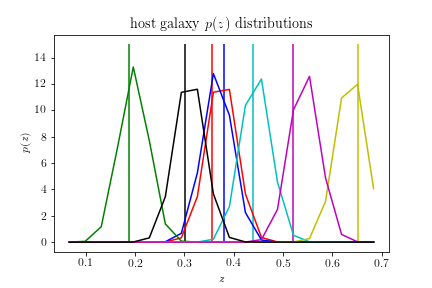
\includegraphics[width=0.5\textwidth]{fig/host_likelihoods.png}
		\caption{These are examples of mock photo-$z$ posteriors.  \textbf{(@aimalz Change these to plot as piecewise constant.)}}
		\label{fig:pzs}
	\end{center}
\end{figure}

\subsubsection{Host galaxy redshift analysis model}
\label{sec:hostinterim}

The interim prior $p(z | \vec{\varphi}^{*})$ is a normalized redshift distribution that is often a best guess for that of the survey in question, based on one from a previous survey or training set for a photometric redshift PDF code.  Here, we use that of the Sloan Digital Sky Survey (SDSS) Data Release 7 (DR7) that covers the same redshift range as the redshift-dependent supernova type proportions.  \textbf{(Note: we still need to implement that in code.)}

\subsubsection{Host galaxy selection function}
\label{sec:hostselection}

Though the host galaxy selection function $p(\vec{f} | \vec{\beta})$ is defined in the space of host galacxy photometry $\vec{f}$, it is projected into redshift space as $p(z | \vec{\beta})$.  \textbf{(Note: we have not actually done this yet!)}  The \texttt{Buzzard} simulation produces a catalog of galaxy redshifts, spectral energy distributions (SEDs), photometric magnitudes, and signal-to-noise rates.  Knowing the magnitude limits and signal-to-noise cuts of LSST's WFD and DDF survey strategies, we can calculate the recovery fraction as a function of redshift and SED under each.  (At this point, we could impose a prior on SED due to the known correlation between a galaxy's SED and the type of supernova likely to occur in it, although we do not include that complication in this study.)  We integrate these fractions over SED and take the ratio as
\begin{equation}
    \label{eq:hostselfunwords}
    p(z | \vec{\beta}) = \frac{\frac{\mathrm{number\ of\ recovered\ galaxies\ at\ redshift\ }z\mathrm{\ in\ WFD}}{\mathrm{number\ of\ simulated\ galaxies\ at\ redshift\ }z\mathrm{\ in\ WFD}}}{\frac{\mathrm{number\ of\ recovered\ galaxies\ at\ redshift\ }z\mathrm{\ in\ DDF}}{\mathrm{number\ of\ simulated\ galaxies\ at\ redshift\ }z\mathrm{\ in\ DDF}}}
\end{equation}
to obtain $p(z | \vec{\beta})$.

% \subsection*{Constructing PDFs}
% \label{sec:pdfs}

% The catalog of trios of true latent variables must be transformed into three-dimensional probability distribution functions (PDFs) over these three variables.  To improve the efficiency of \scippr, we use a binned parametrization for the PDFs $p(\mu_{n}, z_{n}, t_{n} | \textul{\ell}_{n}, \vec{f}_{n}, \vec{\theta}, \textul{\xi}, \vec{\alpha}, \vec{\beta})$ so that the mathematical manipulations of the PDFs are simple operations on arrays.  This choice is made at the level of writing code, not something intrinsic to the model.  For these tests, we use $J=20$ equally spaced bins in redshift and $K=20$ equally spaced bins in distance modulus.  

% We construct the PDFs from simple components described in the following sections, guided by the graphical model of Fig. \ref{fig:pgm}.  We will be assuming separability of the data 

% We will discuss the two terms separately. The first term of Eq. \ref{eq:mockBayes} may easily be reduced to $p(\textul{\ell}_{n}, \vec{m}_{n} | \mu_{n}, z_{n}, t_{n})$, as there is no direct dependence of the data on the hyperparameters.  Fig. \ref{fig:pgm} tells us how to break it up, resulting in Eq. \ref{eq:first}.
%
% \begin{align}
% \label{eq:first}
% p(\textul{\ell}_{n}, \vec{m}_{n} | \mu_{n}, z_{n}, t_{n}) &= p(\textul{\ell}_{n} | \mu_{n}, z_{n}, t_{n})\ p(\vec{m}_{n} | z_{n})
% \end{align}
%
% According to Fig. \ref{fig:pgm}, we have Eq. \ref{eq:second}.
%
% \begin{align}
% \label{eq:second}
% p(\mu_{n}, z_{n}, t_{n} | \vec{\theta}^{*}, \textul{\phi}^{*}) &= p(\mu_{n} | z_{n}, \vec{\theta}^{*})\ p(z_{n}, t_{n} | \textul{\phi}^{*})
% \end{align}
%
% These two terms will be addressed separately in Secs. \ref{sec:likelihoods} and \ref{sec:posteriors}.

% \subsubsection*{Creating posteriors}
% \label{sec:posteriors}

% The first components we must construct are the posterior distributions $p(\mu_{n}, z_{n}, t_{n} | \textul{\ell}_{n}, \vec{f}_{n})$.  We note the statistical independence of $\textul{\ell}_{n}$ and $\vec{f}_{n}$, as there are no direct connections between them in Fig. \ref{fig:pgm}.  Furthermore, while the supernova lightcurve is a function of all three latent variables, the host galaxy photometry is independent of the distance modulus and supernova type according to the model of Fig. \ref{fig:pgm}.  (Though there is some evidence against this assumption, the details of any potential relationship have not yet been determined well enough to model, so we do not include this effect at this time.)  Because of these instances of independence, we may decompose the posterior as
% \begin{align}
% \label{eq:posteriors_decompose}
% p(\mu_{n}, z_{n}, t_{n} | \textul{\ell}_{n}, \vec{f}_{n}) &= p(\mu_{n}, z_{n}, t_{n} | \textul{\ell}_{n})\ p(z_{n} | \vec{f}_{n}).
% \end{align}
% We construct these terms without simulating supernova lightcurves nor host galaxy photometry.  The true supernova types, redshifts, and distance moduli serve as a proxy for the information that would be carried by the observed data; in other words, we are saying
% \begin{align}
% \label{eq:posteriors_emulate}
% p(\mu_{n}, z_{n}, t_{n} | \textul{\ell}_{n}, \vec{f}_{n}) &= p(\mu_{n}, z_{n}, t_{n} | \mu'_{n}, z'_{n}, t'_{n})\ p(z_{n} | z'_{n}).
% \end{align}
% We thus emulate the desired posteriors based on our understanding of the forward model of point estimates of these quantities.

% We first approach the second term, the photo-$z$ posterior.  The piecewise constant parametrization is flexible enough to accommodate many shapes for the redshift posterior, but for now, we assume it is a binned Gaussian distribution $\mathcal{N}(z_{n}''^{f}, \sigma_{f}^{2})$ with a variance $\sigma_{f}^{2}$ shared by the entire dataset and a mean of $z_{n}''^{f}$ drawn from a Gaussian distribution $\mathcal{N}(z'_{n}, \sigma_{f}^{2})$ of the same variance with a mean of $z'_{n}$, the true redshift.  Examples of these photo-$z$ posteriors are shown in Fig. \ref{fig:pzs}.

% \begin{figure}
% 	\begin{center}
% 		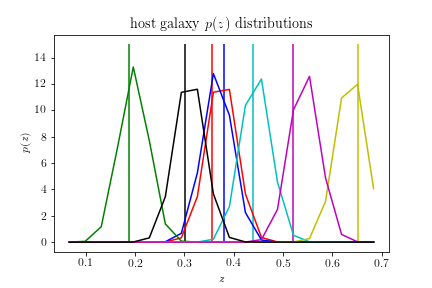
\includegraphics[width=0.5\textwidth]{fig/host_likelihoods.png}
% 		\caption{These are examples of mock photo-$z$ posteriors.  \textbf{(@aimalz Change these to plot as piecewise constant.)}}
% 		\label{fig:pzs}
% 	\end{center}
% \end{figure}

% The first term is more challenging due to its higher dimensionality.  We are modeling the expected product of a probabilistic lightcurve fitter that gives a joint probability distribution over supernova type, redshift, and distance modulus.  As this is an emulation procedure, rather than a simulation, we construct the desired quantity using an understanding of how a lightcurve fitter works.  Depending on the type of supernova, a different fitting function is used, so typically a classifier is run on the lightcurves first, and then that information is fed into a lightcurve fitter.  This is equivalent to
% \begin{align}
% \label{eq:lc_fit_model}
% p(\mu_{n}, z_{n}, t_{n} | \mu'_{n}, z'_{n}, t'_{n}) &= p(t_{n} | t'_{n})\ p(\mu_{n}, z_{n} | \mu'_{n}, z'_{n}, t'_{n}, t_{n}).
% \end{align}

% The quantity $p(t | t'_{n})$ is a vector of length $T$ in which each cell is the probability of a supernova's classified type given its true type, evaluated at the true type $t'_{n}$ of supernova $n$.  The $T\times T$ matrix defined by $p(t | t')$ is called the confusion matrix $\textul{C}$ of a classifier, whose diagonal elements give the fraction of supernovae classified as their true type.  \textbf{(We need to choose a confusion matrix typical of a modern classifier and use that in the tests.)}

% We motivate the mechanism producing $p(\mu_{n}, z_{n} | \mu'_{n}, z'_{n}, t'_{n}, t_{n})$.  We currently assume that this function is separable into a redshift-dependent component $p(z_{n} | z'_{n})$ and a redshift-independent component $p(\mu_{n} | \mu'_{n}, t'_{n}, t_{n})$.  \textbf{(We can and should revise this assumption.  @reneehlozek Where can we find information upon which to base a better emulation model?)}  For these, we use the same model as for the redshift posteriors based on host galaxy photometry, with a variance $\sigma_{\ell}^{2}$ and mean $z_{n}''^{\ell}$, yielding a vector of length $J$.

% When constructing a traditional Hubble diagram, we only attempt to estimate a distance modulus for type Ia supernovae, leaving the distance modulus of non-standardizable types unconstrained.  This choice is based on the classified type $t_{n}$ rather than the true type.  When there is a misclassification, i.e. $t_{n}\neq t'_{n}$, a type Ia supernova might be given an unconstrained distance modulus and a core-collapse supernova would be assigned systematically incorrect distance modulus.  In particular, type II contaminants tend to have a high scatter around a constant distance modulus and type Ibc contaminants tend to be systematically biased to lower distance moduli.  \textbf{(We need to find one of those figures showing these functions!)}  Based on these observations, we establish functions $p(\mu_{n} | \mu'_{n}, t'_{n}, t_{n})$ corresponding to all elements of the confusion matrix and evaluate them at the known values of $\mu'_{n}$ and $t'_{n}$ and each possible value of $t_{n}$, yielding a $T\times K$ matrix for each supernova in the sample. 
% To simulate the values of the distance modulus and type we use
% \begin{eqnarray}
% \label{eq:emulation}
% p(\mu_{n} | \mu'_{n}, t'_{n}=Ia, t_{n}=Ia) &=& \mathcal{N}(\mu''_{n}, \sigma_{Ia}^{2}); \nonumber \\ &&\mu''_{n}\sim\mathcal{N}(\mu'_{n}, \sigma_{Ia}^{2}) \nonumber \\
% p(\mu_{n} | \mu'_{n}, t'_{n}=Ibc, t_{n}=Ia) &=& \mathcal{N}(\mu''_{n}, \sigma_{Ibc}^{2}); \nonumber \\  &&\mu''_{n}\sim\mathcal{N}(\mu'_{n} - c_{Ibc}, \sigma_{Ibc}^{2})\nonumber \\
% p(\mu_{n} | \mu'_{n}, t'_{n}=II, t_{n}=Ia) &=& \mathcal{N}(\mu''_{n}, \sigma_{II}^{2}); \nonumber \\ &&\mu''_{n}\sim\mathcal{N}(c_{II}, \sigma_{II}^{2})\nonumber \\
% p(\mu_{n} | \mu'_{n}, t'_{n}, t_{n}\neq Ia) &=& U(\mu_{min}, \mu_{max}), \nonumber \\
% \end{eqnarray}
% where $c_{Ibc}$ and $c_{II}$ are constants shared among all supernovae.

% \subsubsection*{Incorporating the selection function}
% \label{sec:selectionfunctions}

% So far, we have not considered the effect of selection functions in the space of observed supernova lightcurves and host galaxy photometry, though they are obviously very important.  We assume that the survey producing the catalog of three-dimensional posteriors knows its selection functions in the space of data, which correspond to $p(\textul{\ell} | \vec{\alpha})$ and $p(\vec{f} | \vec{\beta})$.  Given models for the relationships between data and latent variables $p(\mu, z, t | \textul{\ell})$ and $p(z | \vec{f})$, we could marginalize over the space of all possible data to obtain $p(\mu, z, t | \vec{\alpha})$ and $p(z | \vec{\beta})$, which would then simply be multiplied to get $p(\mu, z, t | \vec{\alpha}, \vec{\beta})$.  

% Because we do not simulate the supernova lightcurves nor host galaxy photometry, this approach is not available to us.  Once again, we will emulate it, this time using summary statistics of mock data from realistic simulations.  We can calculate the recovery rate in the space of latent variables given different selection function parameters by actually imposing those selection functions on realistic simulations for which the true distribution in the space of $\mu$, $z$, and $t$ is known. 

% In the simple case of host galaxy photometry, we assume the cuts in magnitude and signal-to-noise ratio expected of LSST and apply these to the photometry of the Buzzard catalog with a known redshift distribution.  By simply taking the ratio of recovered galaxies to simulated galaxies within each of the $J$ redshift bins.  Note that we have already assumed no correlation between host galaxy properties and supernova type, but if there were a simulation that accurately included this effect, we could obtain a selection function in the space of $t$ and $z$ based on that.  \textbf{(We need to actually do this with realistic cuts and mock data.)}  This procedure gives us $p(z | \vec{\beta})$.

% In the three-dimensional case of supernova lightcurves, there is not a mock dataset with information on the true number of supernovae at each $\mu$, $z$, and $t$.  \textbf{(Is this the nominal reason why we have to take the ratio of what's recovered with the WFD selection cuts to what's recovered with the DDF selection cuts?  I don't understand how we have either of those numbers if that data is not available.  Is it because the recovery rate requires choosing a classifier and lightcurve fitter?)}  Instead of using the ratio of the number of supernovae recovered over the number of supernovae simulated as a function of their latent variables, we use the ratio of the recovery rate for the selection function in question over the recovery rate for the most generous possible selection function.  For LSST, these correspond to the Wide Fast Deep (WFD) and Deep Drilling Fields (DDF) selection functions.  This procedure gives us $p(z, t | \vec{\alpha})$.  The selection function on $\mu$ is cosmology-dependent so is not included in this model.  \textbf{(Should we try to include this or assert that given a cosmology, it is a straightforward result of $p(z, t | \vec{\alpha})$?)}

% The product of the selection function terms $p(z | \vec{\beta})$ and $p(z, t | \vec{\alpha})$ gives us the overall selection function term $p(\mu, z, t | \vec{\alpha}, \vec{\beta})$.

% \subsubsection*{Making interim posteriors}
% \label{sec:interimpriors}

% Recall the interim priors introduced in Sec. \ref{sec:model}.  The way they enter the production of interim posteriors is functionally equivalent to the selection functions.  Rather than arising from biases in the collection of the observed data, the interim priors result from the method by which the observed data is converted into estimates of the posteriors of Sec. \ref{sec:posteriors}.  Examples would be the bias due to the choice of training set for a machine learning method or the presumed distribution of the latent variables in a template-fitting approach.  So long as the interim priors are known, we can still perform an unbiased inference.  We model the interim priors separately for the production of photo-$z$ PDFs and the three-dimensional posteriors from the lightcurves.  

% The interim prior for a photo-$z$ PDF method is a form of $p(z | \vec{\theta})$, the redshift distribution conditioned on a known set of parameters.  Given our piecewise constant parametrization of redshift space, we can take $\vec{\theta}$ to be comprised of probabilities over each bin.  We choose it to mimic the redshift distribution from a previous spectroscopic survey.  \textbf{(Currently it's flat, but it would be reasonable to use the SDSS DR8 $n(z)$ as an interim prior.)}

% The interim prior for our anticipated probabilistic lightcurve fitter must be a distribution in the three-dimensional space of latent variables.  Here, we choose the interim prior parameters comprising $\textul{\xi}$ to be the cosmological parameters from a previous study and their error estimates, as well as a uniform redshift-independent supernova type proportion.  The cosmological parameters and their error bars correspond to a probability density over the Hubble diagram, which can be expressed as a piecewise constant function in the two-dimensional space of redshift and distance modulus.  The uniform interim prior on supernova types indicates that there will be $T$ identical $J\times K$ element matrices comprising the probability distribution $p(\mu, z, t | \textul{\xi})$.

%Because the parametrization hasn't changed, the term $p(z_{\zeta}, t_{\tau} | \textul{\phi}^{*})$ takes the simple form of $\phi^{*}_{\tau\zeta}$.  Similarly, $p(\mu_{\nu} | z_{\zeta}, \vec{\theta}^{*})$ will be a delta function $\delta_{f_{\vec{\theta}^{*}}(z_{\zeta})}(\mu_{\nu})$.  
%
%Finally, in Eq \ref{eq:interimposteriordata}, we put these pieces together to express the form of the individual interim posteriors of the form of Eq. \ref{eq:mockBayes}.
%
%\begin{align}
%\label{eq:interimposteriordata}
%p_{n}(\mu_{\nu}, z_{\zeta}, t_{\tau} | \textul{\ell}_{n}, \vec{m}_{n}, \vec{\theta}^{*}, \textul{\phi}^{*}) &= KC_{\tau'_{n}\tau}\mathcal{N}_{(\hat{z}^{\ell}, \hat{\mu}^{\ell}), \textul{\Sigma}_{n}}(z_{\zeta}, \mu_{\nu}) \mathcal{N}_{\hat{z}_{n}^{m}, \sigma_{n}^{2}}(z_{\zeta}) \phi^{*}_{\zeta\tau}\delta_{f_{\vec{\theta}^{*}}(z_{\zeta})}(\mu_{\nu})
%\end{align}
%
%The constant of proportionality $K$ here will be set such that $\sum_{\nu}^{D}\sum_{\zeta}^{Z}\sum_{\tau}^{T} p_{n}(\mu_{\nu}, z_{\zeta}, t_{\tau} | \textul{\ell}_{n}, \vec{m}_{n}, \vec{\theta}^{*}, \textul{\phi}^{*})=1$.

\subsection{Mock data product}
\label{sec:finalmockdata}

Finally, we have all the components necessary to 

\section{Results \& Discussion}
\label{sec:results}

\section{Conclusion \& Future Directions}
\label{sec:conclusion}

%\acknowledgments

%\appendix

\bibliography{references}
\begin{strip}
\begin{appendix}
\label{appendix:derivation}

Starting with Equation~\ref{eq:independence}, we marginalize over the latent variables, showing how the unobservable variables enter the inference:
\begin{align}
\label{eq:marginalization}
p(\textul{\ell}_{n}, \vec{f}_{n} | \vec{\Omega}, \textul{\phi}) &= \iiint p(\textul{\ell}_{n}, \vec{f}_{n} | \mu_{n}, z_{n}, t_{n})\ p(\mu_{n}, z_{n}, t_{n} | \vec{\Omega}, \textul{\phi})\ d\mu_{n}\ dz_{n}\ dt_{n}
\end{align}
 
  We note that Eq. \ref{eq:marginalization} calls for the likelihoods $\{p(\textul{\ell}_{n}, \vec{f}_{n} | \mu_{n}, z_{n}, t_{n})\}_{N}$ containing the supernova lightcurve and host galaxy photometry \textit{given} some particular values of distance modulus, redshift, and type. What we have at our disposal are the \textit{interim posteriors}  $\{p(\mu_{n}, z_{n}, t_{n} | \textul{\ell}_{n}, \vec{f}_{n}, \vec{\theta}, \textul{\xi}, \vec{\alpha}, \vec{\beta})\}_{N}$, which are probabilities of the distance modulus, redshift, and type given fixed values for the supernova lightcurve, host galaxy photometry, and priors from the data analysis procedure and survey program.

We thus must transform our expression Eq.~\ref{eq:marginalization} to be in terms of quantities at our disposal. This is achieved by multiplying the likelihood by an inspired factor of unity, in terms of the interim posteriors.
\begin{align}
\label{eq:unity}
p(\textul{\ell}_{n}, \vec{f}_{n} | \mu_{n}, z_{n}, t_{n}) &= p(\textul{\ell}_{n}, \vec{f}_{n} | \mu_{n}, z_{n}, t_{n})\ \frac{p(\mu_{n}, z_{n}, t_{n} | \textul{\ell}_{n}, \vec{f}_{n},\vec{\theta}, \textul{\xi}, \vec{\alpha}, \vec{\beta})}{p(\mu_{n}, z_{n}, t_{n} | \textul{\ell}_{n}, \vec{f}_{n}, \vec{\theta}, \textul{\xi}, \vec{\alpha}, \vec{\beta})}
\end{align}
We expand the denominator of the fraction on the right hand side according to Bayes' Rule: $p(\mu_{n}, z_{n}, t_{n} | \textul{\ell}_{n}, \vec{f}_{n}, \vec{\theta}, \textul{\xi}, \vec{\alpha}, \vec{\beta}) = p(\mu_{n}, z_{n}, t_{n} | \vec{\theta}, \textul{\xi}, \vec{\alpha}, \vec{\beta})\ p(\textul{\ell}_{n}, \vec{f}_{n} | \mu_{n}, z_{n}, t_{n}, \vec{\theta}, \textul{\xi}, \vec{\alpha}, \vec{\beta})$ to obtain (\textbf{RH: we don't describe how a term was added to the numerator here})

\begin{align}
\label{eq:expand}
p(\textul{\ell}_{n}, \vec{f}_{n} | \mu_{n}, z_{n}, t_{n}) &= p(\textul{\ell}_{n}, \vec{f}_{n} | \mu_{n}, z_{n}, t_{n})\ p(\mu_{n}, z_{n}, t_{n} | \textul{\ell}_{n}, \vec{f}_{n},\vec{\theta}, \textul{\xi}, \vec{\alpha}, \vec{\beta})\ \frac{p(\textul{\ell}_{n}, \vec{f}_{n} | \vec{\theta}, \textul{\xi}, \vec{\alpha}, \vec{\beta})}{p(\mu_{n}, z_{n}, t_{n} | \vec{\theta}, \textul{\xi}, \vec{\alpha}, \vec{\beta})\ p(\textul{\ell}_{n}, \vec{f}_{n} | \mu_{n}, z_{n}, t_{n}, \vec{\theta}, \textul{\xi}, \vec{\alpha}, \vec{\beta})}
\end{align}
The most daunting term in the denominator of the above can be simplified using the independence of hierarchical models as:
\begin{align}
\label{eq:breakdown}
p(\textul{\ell}_{n}, \vec{f}_{n} | \mu_{n}, z_{n}, t_{n}, \vec{\theta}, \textul{\xi}, \vec{\alpha}, \vec{\beta}) &= p(\textul{\ell}_{n}, \vec{f}_{n} | \mu_{n}, z_{n}, t_{n})\ p(\textul{\ell}_{n}, \vec{f}_{n} | \vec{\theta}, \textul{\xi}, \vec{\alpha}, \vec{\beta}).
\end{align}
Noting the presence of $p(\textul{\ell}_{n}, \vec{f}_{n} | \mu_{n}, z_{n}, t_{n})$ and $p(\textul{\ell}_{n}, \vec{f}_{n} | \vec{\theta}, \textul{\xi}, \vec{\alpha}, \vec{\beta})$ in both the numerator and denominator for $p(\textul{\ell}_{n}, \vec{f}_{n} | \mu_{n}, z_{n}, t_{n})$, we cancel the like terms to express the individual likelihoods in terms of known quantities, obtaining
\begin{align}
\label{eq:cancellation}
p(\textul{\ell}_{n}, \vec{f}_{n} | \mu_{n}, z_{n}, t_{n}) &= \frac{p(\mu_{n}, z_{n}, t_{n} | \textul{\ell}_{n}, \vec{f}_{n}, \vec{\theta}, \textul{\xi}, \vec{\alpha}, \vec{\beta})}{p(\mu_{n}, z_{n}, t_{n} | \vec{\theta}, \textul{\xi}, \vec{\alpha}, \vec{\beta})}.
\end{align}
We are now ready to plug the individual likelihoods into Eq. \ref{eq:marginalization}, leading to
\begin{align}
\label{eq:buildup}
p(\textul{\ell}_{n}, \vec{f}_{n} | \vec{\theta}, \textul{\phi}) &= \iiint p(\mu_{n}, z_{n}, t_{n} | \textul{\ell}_{n}, \vec{f}_{n}, \vec{\theta}^{*}, \textul{\phi}^{*})\ \frac{p(\mu_{n}, z_{n}, t_{n} | \vec{\theta}, \textul{\phi})}{p(\mu_{n}, z_{n}, t_{n} | \vec{\theta}^{*}, \textul{\phi}^{*})}\ d\mu_{n}\ dz_{n}\ dt_{n}
\end{align}
Finally, we plug Eq. \ref{eq:buildup} back into Eq. \ref{eq:independence}.
\begin{align}
\label{eq:plugin}
p(\{\textul{\ell}_{n}, \vec{f}_{n}\}_{N} | \vec{\Omega}, \textul{\phi}) &= \prod_{n}^{N}\ \iiint p(\mu_{n}, z_{n}, t_{n} | \textul{\ell}_{n}, \vec{f}_{n}, \vec{\theta}, \textul{\xi}, \vec{\alpha}, \vec{\beta})\ \frac{p(\mu_{n}, z_{n}, t_{n} | \vec{\Omega}, \textul{\phi})}{p(\mu_{n}, z_{n}, t_{n} | \vec{\theta}, \textul{\xi}, \vec{\alpha}, \vec{\beta})}\ d\mu_{n}\ dz_{n}\ dt_{n}
\end{align}
And finally, we plug the product back into Eq. \ref{eq:bayes} to obtain
\begin{align}
\label{eq:wrapup}
p(\vec{\Omega}, \textul{\phi} | \{\textul{\ell}_{n}, \vec{f}_{n}\}_{N}) &\propto p(\vec{\Omega}, \textul{\phi})\ \prod_{n}^{N}\ \iiint p(\mu_{n}, z_{n}, t_{n} | \textul{\ell}_{n}, \vec{f}_{n}, \vec{\theta}, \textul{\xi}, \vec{\alpha}, \vec{\beta})\ \frac{p(\mu_{n}, z_{n}, t_{n} | \vec{\Omega}, \textul{\phi})}{p(\mu_{n}, z_{n}, t_{n} | \vec{\theta}, \textul{\xi}, \vec{\alpha}, \vec{\beta})}\ d\mu_{n}\ dz_{n}\ dt_{n},
\end{align}
the posterior on cosmological parameters and redshift-dependent type proportions that we wish to sample, which is given as \Eq.~\ref{eq:wrapupmain} in the main body of the paper.
\end{appendix}
\end{strip}


\end{document}